%%%%%%%%%%%%%%%%%%%%%%%%%%%%%%%%%%%%%%%%%%%%%%%%%%%%%%%%%%%%%%%%%%%%%%%
% Sample template for MIT Junior Lab Student Written Summaries
% Available from http://web.mit.edu/8.13/samplepaper/sample-paper.tex
%
% Last Updated June 20, 2004
%
% Adapted from the American Physical Societies REVTeK-4 Pages
% at http://publish.aps.org
%
% ADVICE TO STUDENTS: Each time you write a paper, start with this
%    template and save under a new filename.  If convenient, don't
%    erase unneeded lines, just comment them out.  Often, they
%    will be useful containers for information.
%%%%%%%%%%%%%%%%%%%%%%%%%%%%%%%%%%%%%%%%%%%%%%%%%%%%%%%%%%%%%%%%%%%%%%%


%%%%%%%%%%%%%%%%%%%%%%%%%%%%%%%%%%%%%%%%%%%%%%%%%%%%%%%%%%%%%%%%%%%%%%%
% PREAMBLE
% The preamble of a LaTeX document is the set of commands that precede
% the \begin{document} line.  It contains a \documentclass line
% to load the REVTeK-4 macro definitions and various \usepackage
% lines to load other macro packages.
%
% ADVICE TO STUDENTS: This preamble contains a suggested set of
%     class options to generate a ``Junior Lab'' look and feel that
%     facilitate quick review and feedback from one's peers, TA's
%     and section instructors.  Don't make substantial changes without
%     first consulting your section instructor.
%%%%%%%%%%%%%%%%%%%%%%%%%%%%%%%%%%%%%%%%%%%%%%%%%%%%%%%%%%%%%%%%%%%%%%%

\documentclass[aps,twocolumn,secnumarabic,nobalancelastpage,amsmath,amssymb,
nofootinbib]{revtex4}

% nofootinbib is another document class option that allows you to put
% footnotes on the page where they occur rather than at the end of the
% paper.  This makes for easier reading!

% secnumarabic is a particularly nice way of identifying sections by
% number to aid electronic review and commentary.

% amsmath and amssymb are necessary for the subequations environment
% among others

\usepackage{graphics}      % standard graphics specifications
\usepackage{graphicx}      % alternative graphics specifications
\usepackage{longtable}     % helps with long table options
\usepackage{url}           % for on-line citations
\usepackage{bm}            % special 'bold-math' package
\usepackage{subfigure}
\usepackage{booktabs}

%%%%%%%%%%%%%%%%%%%%%%%%%%%%%%%%%%%%%%%
%                                 %%%%%
% And now, begin the document...  %%%%%
%                                 %%%%%
%%%%%%%%%%%%%%%%%%%%%%%%%%%%%%%%%%%%%%%
\begin{document}
\title{Rutherford Scattering}
\author         {Kevin L. Chen. Partner: Tanooj Shah}
\affiliation    {UC Berkeley, Department of Physics}
\date{\today}

\begin{abstract}
% Do at the end
\end{abstract}

\maketitle

%%%%%%%%%%%%%%%%%%%%%%%%%%%%%%%%%%%%%%%%%%%%%%%%%%%%%%%%%%%%%%%%%%%%%%%%%%%%%
\section{Introduction}

Atomic Spectroscopy is one of the fundamental fields of physics where Quantum Mechanics its energy level became more robust theoretically. From atomic spectroscopy, physicists have discovered the Rydberg Formula, illustrating the transitions between electron energy levels. One of the most important of these transitions are called the Balmer Series, which depicts the transitions from n > 3 states to n = 2 stages. The light from this series is visible light. Furthermore, by introducing a magnetic field to the atom, we add a new term to the Hamiltonian. This new term gives rise to Zeeman splitting. With this magnetic field, we see spectral lines splitting, due to a split in the energy levels. Using modern day optics and spectroscopic techniques, we can use these spectral lines to determine the Rydberg Constant and the Bohr Magneton. 
%%%%%%%%%%%%%%%%%%%%%%%%%%%%%%%%%%%%%%%%%%%%%%%%%%%%%%%%%%%%%%%%%%%%%%%%%%%%%
\section{Theory}
\subsection{Balmer Series}

To begin speaking about the Balmer Series, one must understand the Bohr Model. In this mode of an atom, the electron revolves around the nucleus of the atom, much like a planet revolves around the sun. Therefore, we have a force balance equation 

\begin{equation}
    {m_\mathrm{e} v^2\over r} = {Zk_\mathrm{e} e^2 \over r^2} 
   \label{Coulomb Force}
\end{equation}

We can find a more specific description of the Coulomb force for the Thomson Model. In the Thomson Model, the positive charge is diffusely spread throughout the atom. For instance, a particle $q$ at position $\boldsymbol{r}$ in a continuous distribution of charge will experience $\boldsymbol{F}$ given by

\begin{equation}
   \boldsymbol{F} = {q\over 4\pi\varepsilon_0}\int dq' {\boldsymbol{r} - \boldsymbol{r'} \over |\boldsymbol{r} - \boldsymbol{r'}|^3}.
   \label{Continuous Coulomb}
\end{equation}

where $dq' = \rho(\boldsymbol{r'})\,dV'$ and where the integral is taken over the volume of the atom.

\begin{figure}[t]
  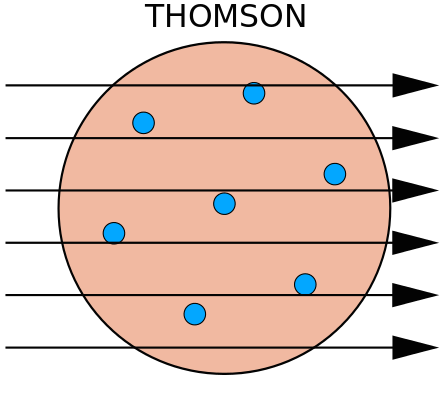
\includegraphics[scale=0.25]{ThomsonRutherford.png}
  \begin{center}
  \caption{Top: The Thomson model of the atom. Bottom: The Rutherford model of the atom.}[\footnotesize{``Atoms.'' Wikipedia. Wikimedia Foundation, n.d. Web. 12 Mar. 2015}]
  \label{ThomsonRutherford}
  \end{center}
\end{figure}

Since the charge will be distributed over the entire atom, then $\rho$ will be much smaller compared to if all the charge was concentrated in a smaller area. In fact, the nucleus has been shown to be on the order 100,000 times smaller than the atom itself (for example, the factor is 23,000 for uranium and 145,000 for hydrogen).

In this experiment, we observe that some alpha particles do in fact experience a very large deflection when passing through gold foil, indicative of a strong Coulomb Force. This strong Coulomb Force must come from a concentration of positive charge, which can be described by Equation~\ref{Discrete Coulomb} rather than Equation~\ref{Continuous Coulomb} if the size of the alpha particle is comparable to the size of the nucleus. 

In this experiment, we are trying to determine the charge of the gold nucleus. In order to do this, we must consider the fraction of particles that scatter as a function of the angle. In Reference~\cite{Melissinos}, A.C. Melissinos derives the differential cross section from knowing the Coulomb Force and scattering mechanics from Classical Theory (see Figure~\ref{ScatteringTheory}). 

\begin{figure}[h]
  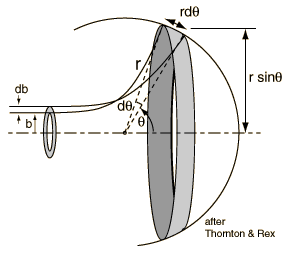
\includegraphics[scale=0.6]{ruthcross.png}
  \begin{center}
  \caption{Depiction of a classical particle being scattered by the Coulomb Force.}[\footnotesize{``Scattering Cross Section.'' HyperPhysics. N.p., n.d. Web. 12 Mar. 2015.}]
  \label{ScatteringTheory}
  \end{center}
\end{figure}

Melissinos begins with the trajectory equation

\begin{equation}
  \frac{d^{2}u}{d\theta^{2}}+u=-\frac{Z_{1}Z_{2}e^{2}}{4\pi\epsilon_{0}mv_{0}^{2}b^{2}}
  \label{StartDerivation}
\end{equation}

with $u={1 \over r}$, $v_0$ as the velocity of the incoming particle at infinity (the velocity of the particle with no interaction with the nucleus), and $b$ as the impact parameter. Through arrives at the final equation 

\begin{equation}
  \frac{d\sigma}{d\Omega}=\left  (\frac{Z_1Z_2e^2}{4E} \right )^2\sin^{-4}{\frac{\theta}{2}}
  \label{DifferentialCrossSection}
\end{equation}    

Furthermore, we will need to find the number of alpha particles scattered into the detector, which is determined in Reference~\cite{Melissinos}:

\begin{equation}
  I_s = I_0 N \frac{d\sigma}{d\Omega} d\Omega
  \label{NumberOfAlphasScattered}
\end{equation}   

where $I_s$ is the counting rate of scattered atoms at a certain angle, $I_0$ is the incident scattering rate, $N$ is the area density of gold foil, and $d\Omega$ is the solid angle of the detector. 

In our experiment, we already have $Z_2$, the atomic number of the alpha particle, and we control the angle $\theta$ of the detector. To find $Z_1$ in Equation~\ref{DifferentialCrossSection}, we must find $\frac{d\sigma}{d\Omega}$, which can be determined by finding the solid angle of the detector aperture and the number of detected particles in an interval of time as a function of angle. This variables are conveniently located in Equation~\ref{NumberOfAlphasScattered}, so by combining Equation~\ref{DifferentialCrossSection} and Equation~\ref{NumberOfAlphasScattered}, we arrive at the final equation we will use to determine the atomic number of gold:

\begin{equation}
  Z_1 = \frac{4E}{Z_2e^2} \sin^{2}{\frac{\theta}{2}} \sqrt{\frac{I_s}{I_0 N d \Omega}}
  \label{FinalEquation}
\end{equation} 

\subsection{Energy Loss}

In this experiment, alpha particles lose energy for two main reasons: interactions with the electron clouds and the passing through the wall of the gun. There are also other reasons for energy loss: Cherenkov radiation, bremsstrahlung, and inelastic nuclear interactions. Before energy loss, the energies of the particles are broken up roughly into three categories: The energies of emitted alpha particles are 5.49 MeV (86\%), 5.44 MeV (13\%), and 5.39 MeV (1.3\%). Due to the brevity of time to conduct and do analysis of this experiment, we will forgo a detailed derivation of the energy loss from these effects. Instead, we will take the average energies of the alpha particles to be 3.77 MeV when they reach the detector. One can go more depth into the details of the energy loss by looking in Reference~\cite{Comfort}.

%%%%%%%%%%%%%%%%%%%%%%%%%%%%%%%%%%%%%%%%%%%%%%%%%%%%%%%%%%%%%%%%%%%%%%%%%%%%%
\section{Set Up}
\subsection{Equipment}

\begin{figure}[htp]
  \begin{center}
    \subfigure[Table Set-up]{\label{Table}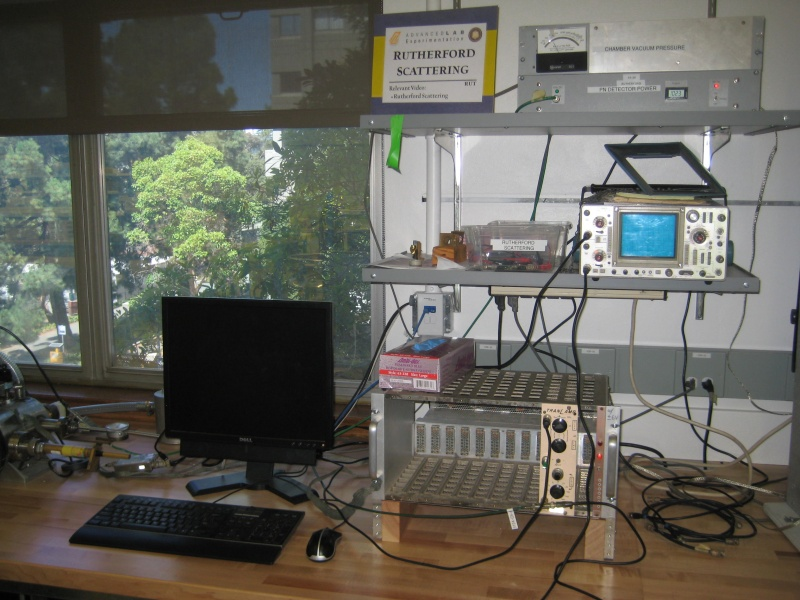
\includegraphics[width=4 cm]{RUT1.jpg}}
    \subfigure[Vacuum Valve]{\label{Valve}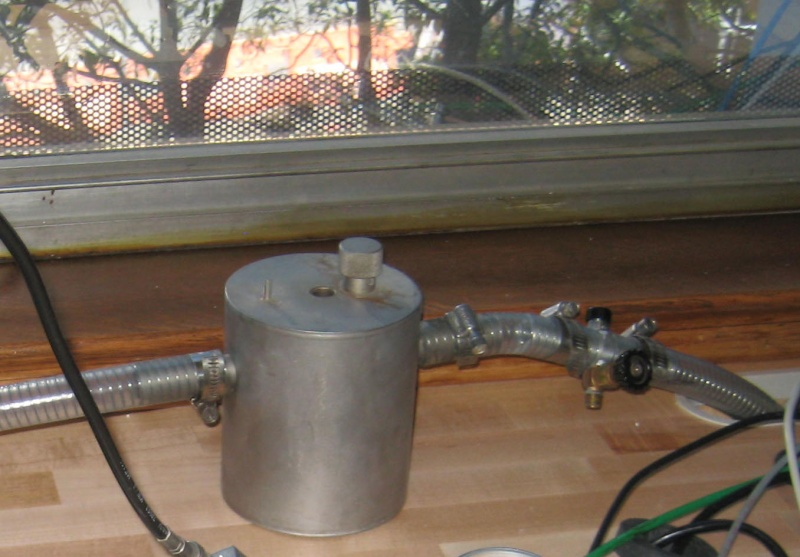
\includegraphics[width=4.3 cm]{RUT2.jpg}} \\
    \subfigure[Scattering Chamber]{\label{Chamber}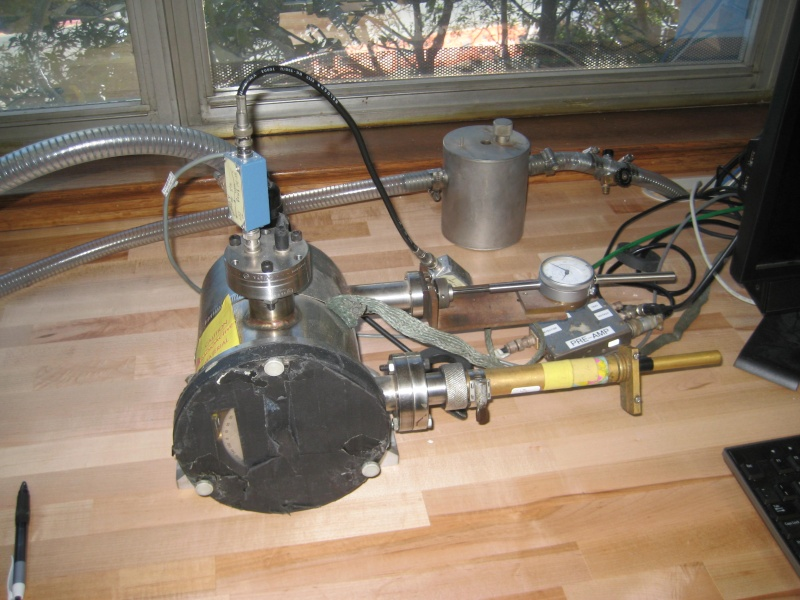
\includegraphics[width=9 cm]{RUT3.jpg}}
  \end{center}
  \caption{Rutherford Experiment Setup at UC Berkeley}[\footnotesize{``Rutherford Scattering.'' - Physics 111-Lab Wiki. UC Berkeley, n.d. Web. 13 Mar. 2015.}]
  \label{ThreeFigs}
\end{figure}

\begin{enumerate}
\item Vacuum Chamber with an adjustable detector and corresponding angle measure to measure the angle between the detector and the axis of the alpha gun. Our detector is a Silicon PN-junction with about 250 microns of gold on it. It has a bias of 50 volts at 4 microamps with a diameter of 0.75 inches. The detector receives its power through a voltage divider to get 50 volts from the 100 volt power supply in the rack
\item An alpha particle source. In our experiment, we used Americium 241. 
\item A gun in which the alpha particle is placed with an adjustable aperture size. The gun was placed 7.8 cm away from the detector. 
\item Double layers of gold leaf foils that can be mounted in front the alpha gun.
\item A vacuum pump.
\item An oscilloscope to detect energy from the alpha gun. 
\item A data taking software. In our experiment, we used a pre-coded LabVIEW program called PHA-5124. This allowed us to measure the energies, counts, and set the gain of energies of the alpha particles that interacts with the detector. 
\item Pre-amp
\item Tran-L-Amp
\end{enumerate}

All equipment can be seen in the figures: Figure~\ref{ThreeFigs}, Figure~\ref{Diagram}, and Figure~\ref{OutisdeDiagram}.

\begin{figure}[h]
  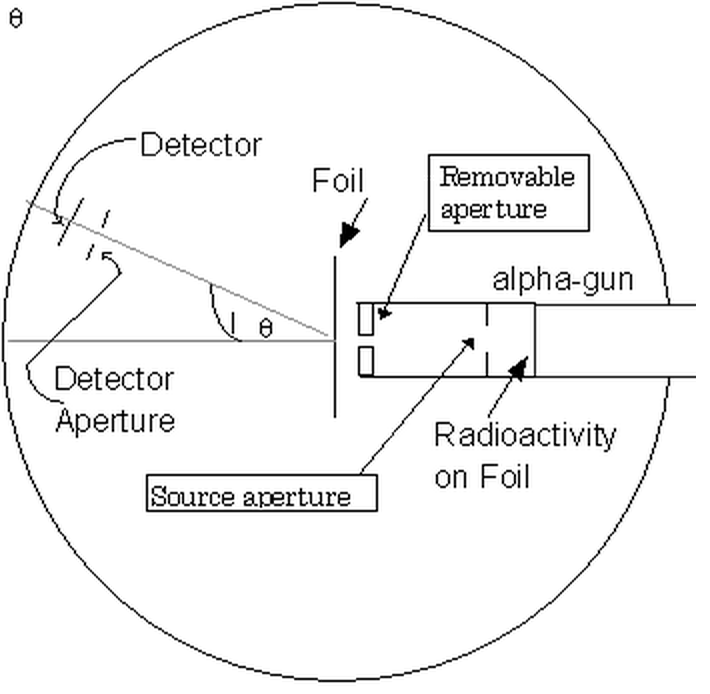
\includegraphics[width = 5 cm]{Diagram.png}
  \begin{center}
  \caption{Inside the vacuum chamber}[\footnotesize{``Rutherford Scattering.'' - Physics 111-Lab Wiki. UC Berkeley, n.d. Web. 13 Mar. 2015.}]
  \label{Diagram}
  \end{center}
\end{figure}

\begin{figure}[h]
  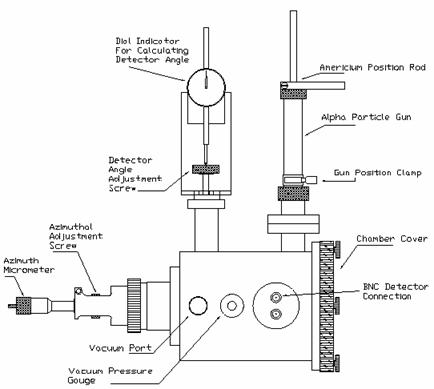
\includegraphics[width = 5 cm]{Diagram2.jpg}
  \begin{center}
  \caption{Outside the vacuum chamber}[\footnotesize{``Rutherford Scattering.'' - Physics 111-Lab Wiki. UC Berkeley, n.d. Web. 13 Mar. 2015.}]
  \label{OutisdeDiagram}
  \end{center}
\end{figure}

\subsection{Taking Measurements}

For our experiment, we first created a vacuum in the chamber. Then we adjusted the Tran-L-Amp to where we set the DIFF to 1.0, INT to 0.05, Coarse Gain to 100, Vennier Gain to  5.9 microseconds, and the FINE GAIN at 1.75. Finally, with the detector at 0 degrees, we make sure that the detector is receiving a signal that displays on the oscilloscope. An example of this signal is in Figure~\ref{Scope}.

\begin{figure}[h]
  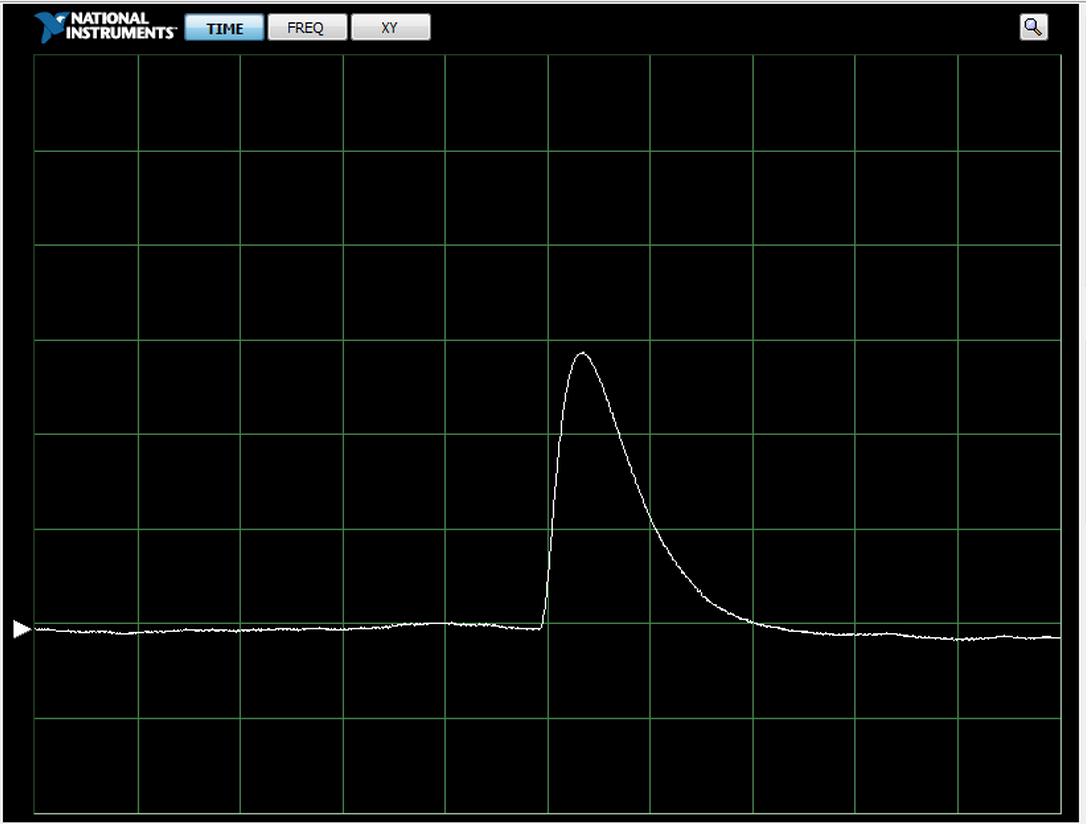
\includegraphics[width = 5 cm]{Scope.png}
  \begin{center}
  \caption{The feed into the scope}[\footnotesize{``Rutherford Scattering.'' - Physics 111-Lab Wiki. UC Berkeley, n.d. Web. 13 Mar. 2015.}]
  \label{Scope}
  \end{center}
\end{figure}

\section{Measurements and Analysis}

when we took measurements, we first took measurements of the intensity of the alpha gun itself, then the angle dependence of the alpha particles without any gold foil, and then finally we included the gold foil and found the angle dependence. 

In Table~\ref{PointBlank} we see the counting rate of the gun at point blank. This is much greater than the maximum counting rate of gun at its default position of 7.8 cm. With that distance, the maximum counting rates were much less than the point blank counting rate. However, we can see from Table~\ref{NoFoilTable} that when the point rates of the angles are summed up, we get near the total counts when we have the gun at point blank. This indicates to us that the alpha particle beam is not emitting straight out of the gun; instead, it had an angular dependence. In the theory we discussed energy loss due to collisions with the walls of the gun. In Table~\ref{Energies}, however, we see that at an angle of 5 degrees, the mean energy is roughly the same for 0 degrees and point blank, and even the distribution in Figure~\ref{EnergiesGraph} looks similar. What is probably happening is that the alpha particle is colliding many times within the gun, and on average, alpha particles are colliding an equal amount of times before exiting the gun. Therefore, the average energy leaving the gun is angle independent. 

We also noticed that in the case of no foil, the counts of alpha particles drops of very quickly past 5 and -5 degrees (see the left plot in Figure~\ref{Combined}). This means that when we insert the gold foil, counts that we receive past 10 and -10 degrees are most likely due to alpha particles scattering off the gold foil.

\begin{table}[h]
\begin{tabular}{|l|l|}
\hline 
Measurement & Count Rate (counts/s)                \\ \hline \hline
Point Blank & 104.84 $\pm$ 10.39                        \\
No Foil, 7.8 cm away from detector & 65.86 Max Value    \\
With Foil, 7.8 cm away from detector & 40.76 Max Value  \\ \hline         
\end{tabular}
\label{PointBlank}
\end{table}

\begin{table}[h]
\begin{tabular}{|l|l|}
\hline
No Foil Angle & Counting Rate (counts/s) \\ \hline \hline
-5            & 4.70                          \\
0             & 65.86                         \\
2.5           & 32.96                         \\
5             & 22.54                         \\
7.5           & 3.863333333                   \\ \hline
\end{tabular}
\label{NoFoilTable}
\end{table}

\begin{table}[h]
\begin{tabular}{|l|l|}
\hline
Angle (Degrees) with No Foil & Energy    \\ \hline \hline
0               & 4.75 $\pm$ 0.74        \\
5               & 4.74 $\pm$ 0.67        \\
Point Blank     & 4.69 $\pm$ 0.94        \\ \hline
\end{tabular}
\label{Energies}
\end{table}

\begin{figure}[h]
  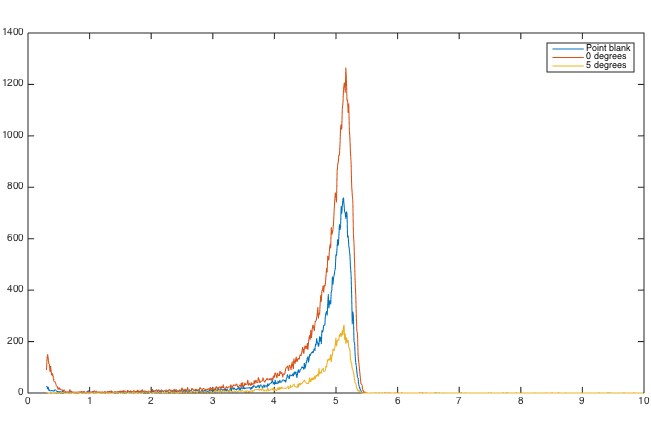
\includegraphics[width = 5 cm]{pointblankcomparison.png}
  \begin{center}
  \caption{Comparison between three configurations without foil.}
  \label{EnergiesGraph}
  \end{center}
\end{figure}


\begin{figure*}[t]
  \includegraphics[width=\textwidth]{Combined Graphs.png}
  \begin{center}
  \caption{Gaussian Fit of angle vs. counting rates for both no foil and with foil}
  \label{Combined}
  \end{center}
\end{figure*}

Now that we've seen how the alpha particles scatter without the gold foil, we can begin looking at the scattering with the gold foil in place. We fit the data to a Gaussian Distribution because the data points looked like they were following a Gaussian curve. Figure~\ref{Combined} shows a wider distribution for the angle, which confirms our theory that gold can scatter alpha particles beyond small angles. For the case of the foil, the standard deviation is 3.94 degrees, which is 48\% larger than 2.66 degrees the standard deviation for no foil. Although there is a difference, this degree of difference is not unexpected, due to the tiny size of the gold nucleus, which is on the order of femtometers. We ought to be seeing a wider spread for the case of the gold foil, but not an absurdly large difference since the small size of the nucleus means that most alpha particles will be deflected a small amount. Large angle deflections would be indicative of alpha particles either coming very close (distance << the size of a gold atom) to one or multiple gold nuclei. 

\begin{table}[h] 
  \begin{tabular}{|l|l|l|}
  \hline
  Measurement & $\mu$ (Degrees) & $\sigma$ of Zero-Position \\ \hline \hline
  No Foil     & 0.1401  (-3.03, 3.311) & 3.761  (0.3299, 7.192)     \\ 
  With Foil   & -0.7366  (-2.407, 0.9333) & 5.568  (2.813, 8.322) \\ \hline     
  \end{tabular}
  \caption{Gaussian Fit of Counting Rate Data (with 95$\%$ confidence bounds)[\footnotesize{Note: Our plot with gold foil also shows an outlying point at 2.5 degrees and large 95$\%$ confidence intervals for the plot for no foil. We will discuss these discrepancies in the error section of our paper.}]}
  \label{ZeroPosition}
\end{table}

\begin{table}[h] 
  \begin{tabular}{|l|l|l|}
  \hline
  Measurement & $\mu$ (Degrees) & Magnitude of Peak (counts/s) \\ \hline \hline
  No Foil     & 0.1401  (-3.03, 3.311) & 61.54  (17.1, 106)    \\ 
  With Foil   & -0.7366  (-2.407, 0.9333) & 29.22  (18.98, 39.46)  \\ \hline     
  \end{tabular}
  \caption{Continuation of Table~\ref{ZeroPosition}
  \label{ZeroPosition2}
\end{table}

Another observation that we made was that the counting rate with the gold foil is less than the counting rate for the case without gold foil. The maximum counting rate near the 0 angle position, according to the Gaussian Fit, was 30 fewer counts/second in the case of the gold foil. This difference is expected due to alpha particles getting scattered outwards from the 0 angle. 


\begin{figure*}[t]
  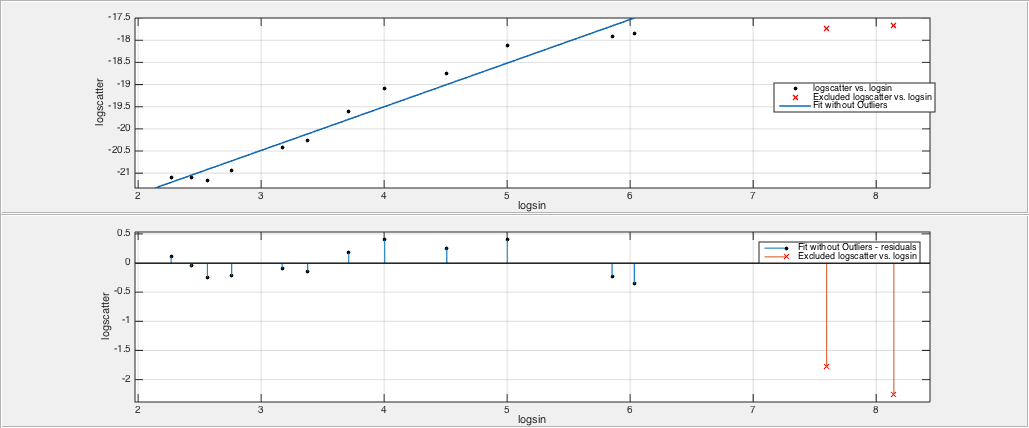
\includegraphics[width=\textwidth]{FitforScatteringCrossSection.png}
  \begin{center}
  \caption{Scattering Cross Section vs. $ \sin(\frac{\theta}{2}))^{-4}$}
  \label{FitforScatteringCrossSection}
  \end{center}
\end{figure*}

With these plots, we can begin to calculate the atomic number of the gold atom. 

\begin{table}[h]
  \begin{tabular}{|l|l|}
  \hline 
  Variable                         & Value               \\ \hline \hline 
  Incident Counting Rate           & 112.19 counts/sec   \\
  Detector Solid Angle             & 0.0060 sr           \\
  Area Density of Gold Foil        & $1.62 * 10^{21} atoms/cm^2$ \\
  Atomic Number of Alpha Particle  & 2                   \\
  Average Energy of Alpha Particle & 3.863333333        \\ \hline
  \end{tabular}
  \label{Values}
\end{table}

\begin{figure}[h]
  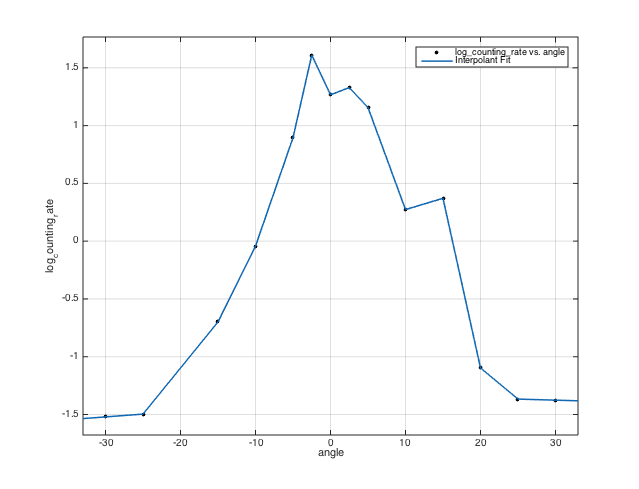
\includegraphics[width=5 cm]{InterpolantFit.png}
  \begin{center}
  \caption{Scattering Cross Section vs. $\sin(\theta))^{-4}$}
  \label{InterpolantFit}
  \end{center}
\end{figure}

% \begin{figure}[t]
%   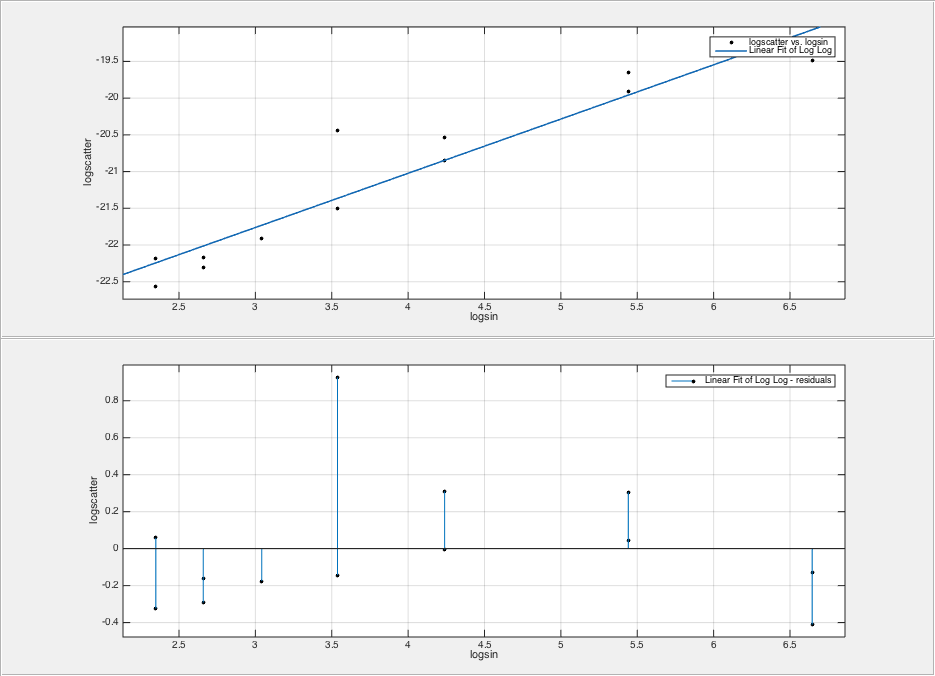
\includegraphics[width = 5 cm]{LinearFitLogLog.png}
%   \begin{center}
%   \caption{Outside the vacuum chamber}
%   \label{OutisdeDiagram}
%   \end{center}
% \end{figure}

% \begin{figure}[t]
%   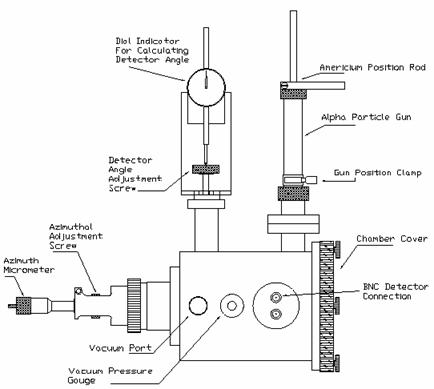
\includegraphics[width = 5 cm]{Diagram2.jpg}
%   \begin{center}
%   \caption{Outside the vacuum chamber}
%   \label{OutisdeDiagram}
%   \end{center}
% \end{figure}


\subsection{Longitudinal Electric Field without a Magnetic Field} 


\subsection{Magnetic Field Strength}


\subsection{The Hall Effect}


\section{Error Discussion}

\begin{figure}[h]
  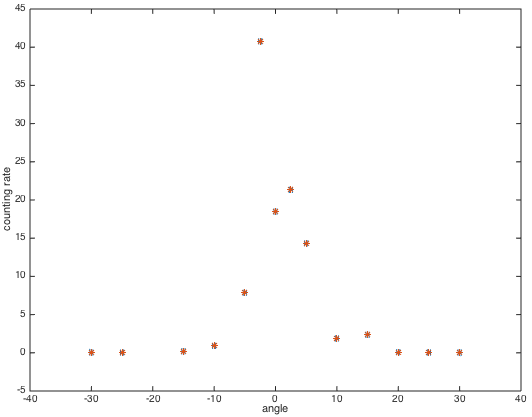
\includegraphics[width=5 cm]{errorfoil.png}
  \begin{center}
  \caption{Error in Angle with Foil}
  \label{ErrorFoil}
  \end{center}
\end{figure}

\begin{figure}[h]
  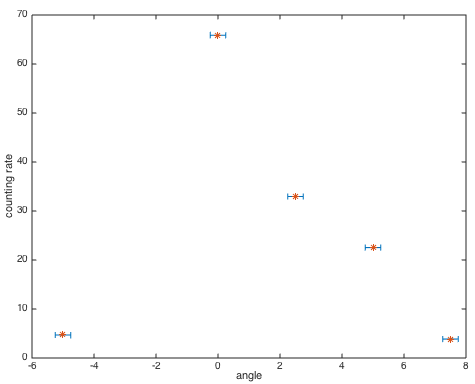
\includegraphics[width=5 cm]{errornofoil.png}
  \begin{center}
  \caption{Error in Angle without Foil}
  \label{ErrorNoFoil}
  \end{center}
\end{figure}

\subsection{Collision Frequency}


\subsection{Electron Drift Velocity and Number Density}



\subsection{Electron Temperature}



\section{Conclusion}



%%%%%%%%%%%%%%%%%%%%%%%%%%%%%%%%%%%%%%%%%%%%%%%%%%%%%%%%%%%%%%%%%%%%%%%%%
% Place all of the references you used to write this paper in a file
% with the same name as following the \bibliography command
%%%%%%%%%%%%%%%%%%%%%%%%%%%%%%%%%%%%%%%%%%%%%%%%%%%%%%%%%%%%%%%%%%%%%%%%%


% %%%%%%%%%%%%%%%%%%%%%%%%%%%%%%%%%%%%%%%%%%%%%%%%%%%%%%%%%%%%%%%%%%%%%%%%%%%%%
\begin{acknowledgments} I acknowledge my lab partner Tanooj Shah for taking data with me and helping me understand the pre-lab questions. I also want to acknowledge Prof Stamper-Kurn for asking challenging questions but ultimately pushing Tanooj and me to truly understand the lab.
\end{acknowledgments}

\begin{thebibliography}{9}

\bibitem{Melissinos}
  A.C. Melissinos, \emph{Experiments in Modern Physics}, Rutherford Scattering, Academic Press Inc. pg. 231-252, 1966

\bibitem{youtube}
  Sumner Davis, \emph{Hall Effect in Plasma}, http://youtu.be/iZkOlZDyb2U, March 7, 2012

\bibitem{Kunkel}
  W. B. Kunkel, \emph{Hall Effect in a Plasma}, American Journal of Physics, Number 733, Volume 49, 1981

\bibitem{website}
  Physics 111 ADV Lab, \emph{Hall Effect in a Plasma}, http://advancedlab.berkeley.edu/, February, 2015

\bibitem{Comfort}
J.R. Comfort, et al., \emph{Energy Loss and Straggling of α Particles in Metal Foils}, Phys. Rev. 150, 249 (1966)

\end{thebibliography}


\end{document}
